\section{Kết quả}\label{sec:results}

\subsection{Các mô hình người học dự báo tốt ngang nhau}\label{sec:res-forecast}

\Cref{tab:forecast} và \cref{fig:forecast} báo cáo dự báo lần nộp đầu cho {{n_T}} người học kiểm tra ({{n_predictions}} dự báo). Sáu mô hình thống kê gần như không phân biệt được: AUC nằm trong khoảng {{auc_dkt2}} đến {{auc_pfa}} và NLL chỉ chênh {{nll_range}}, PFA nhỉnh nhất (NLL {{nll_pfa}}) và DKT ở mức {{nll_dkt}}. Bản song sinh của DKT khớp với bản gốc (NLL {{nll_dkt2}}). Cây định danh đã tỉa kém chính xác hơn (AUC {{auc_id3}}, NLL {{nll_id3}}) nhưng cho ra các luật đọc được; ví dụ, một bài có dưới 30\% người học A vượt qua, được làm bởi người học có tỉ lệ đúng ở lần nộp đầu dưới 40\%, có xác suất đúng dự báo khoảng 0,09--0,10 ở nhiều kỹ năng. Khả năng phân biệt theo kỹ năng tương tự nhau giữa các mô hình (\cref{tab:skills}); các bài con trỏ có AUC thấp nhất và ít quan sát nhất. Nhất quán với các so sánh trước đây \citep{khajah2016deep,wilson2016basics,gervet2020deep}, chỉ riêng độ chính xác dự báo không cho cơ sở nào để ưu tiên một mô hình trong số này làm bộ mô phỏng.

\begin{table}[t]
\centering
\caption{Dự báo lần nộp đầu trên người học giữ lại (mô hình fit trên phân vùng A).}
\label{tab:forecast}
\small
\resizebox{\linewidth}{!}{%
\begin{tabular}{lrcrcrr}
\toprule
Mô hình & AUC & KTC 95\% & NLL & KTC 95\% & Brier & ECE \\
\midrule
{{table_forecast}}
\bottomrule
\end{tabular}}
\par\smallskip
\begin{minipage}{\linewidth}\footnotesize
\textit{Ghi chú.} KTC: khoảng tin cậy 95\% bootstrap theo người học; NLL: log-likelihood âm; ECE: sai số hiệu chỉnh kỳ vọng.
\end{minipage}
\end{table}

\begin{figure}[t]
\centering
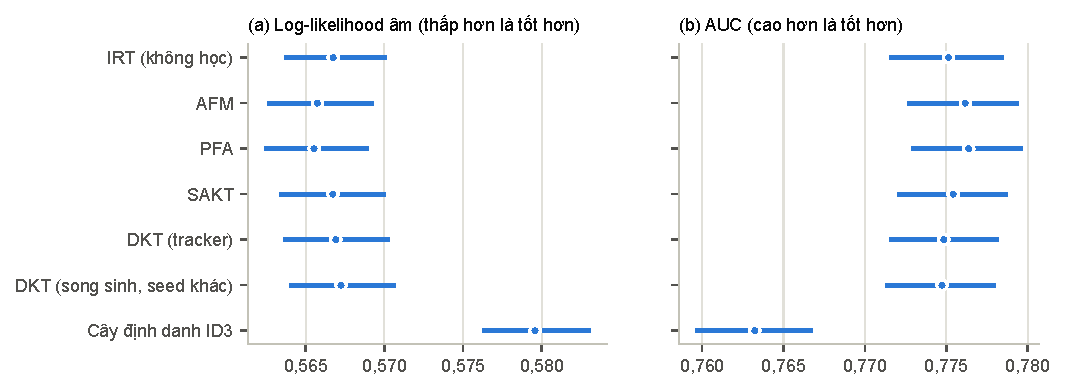
\includegraphics[width=\linewidth]{figures/fig_forecast.pdf}
\caption{Độ chính xác dự báo trên người học giữ lại. (a) Log-likelihood âm và (b) AUC của dự báo lần nộp đầu cho {{n_T}} người học kiểm tra ({{n_predictions}} dự báo); thanh ngang là khoảng tin cậy 95\% bootstrap theo người học. Sáu mô hình thống kê chồng lên nhau; cây định danh dễ diễn giải kém chính xác hơn một chút.}
\label{fig:forecast}
\end{figure}

\subsection{Chính sách trông rất mạnh trong chính bộ mô phỏng huấn luyện}\label{sec:res-insim}

Trong bộ mô phỏng huấn luyện DKT-A, các tác tử thưởng KT cho tiến bộ lớn nhất: PPO nâng post-test kỳ vọng {{insim_ppo_kt}} điểm \% và DQN {{insim_dqn_kt}} điểm \% sau mười bài, so với {{insim_random}} điểm \% của chọn ngẫu nhiên; bộ tối đa hóa tham lam một bước theo tracker đạt {{insim_greedy_kt}} điểm \% (\cref{tab:matrix}). Các tác tử huấn luyện trong thế giới AFM hoặc nhiều thế giới cũng đạt điểm cao trong DKT-A (ví dụ {{insim_dqn_mix}} điểm \% với DQN nhiều thế giới). Nếu đọc riêng lẻ, như thường thấy trong các đánh giá bằng bộ mô phỏng KT, các con số này gợi ý lợi ích lớn của học tăng cường. Tuy nhiên chúng gần như hoàn toàn là độ trôi: trong DKT-A, nơi kết quả do chính tracker sinh ra, phần bất ngờ trong \eqref{eq:decomposition} có trung bình từ {{insim_surprise_min}} đến {{insim_surprise_max}} điểm \% trên {{h3_n}} chính sách (cách 0 tối đa {{insim_surprise_maxz}} sai số chuẩn Monte Carlo; các luồng kết quả ngẫu nhiên được dùng chung giữa các chính sách), trong khi độ trôi tích lũy của PPO là {{insim_drift_ppo_kt}} điểm \%, đúng như \cref{prop:insim} dự đoán (kiểm tra thăm dò).

\begin{table*}[t]
\centering
\caption{Tiến bộ post-test do thế giới đo (điểm \% sau mười bài) của mọi chính sách trong mọi thế giới đánh giá.}
\label{tab:matrix}
\footnotesize
\resizebox{\textwidth}{!}{%
\begin{tabular}{{{matrix_cols}}}
\toprule
Chính sách & {{matrix_header}} \\
\midrule
{{table_matrix}}
\bottomrule
\end{tabular}}
\par\smallskip
\begin{minipage}{\textwidth}\footnotesize
\textit{Ghi chú.} Trung bình trên {{episodes}} lượt đánh giá và, với tác tử học, trên ba seed huấn luyện. $^\dagger$Thế giới huấn luyện. Thế giới DKT và SAKT được đo bằng dự báo của chính chúng; thế giới AFM, PFA và ZPD bằng trạng thái ẩn; IRT-B không có học nên mọi tiến bộ thật bằng 0. Khoảng tin cậy 95\% có trong tệp bổ sung \texttt{evaluation\_matrix\_long.csv}.
\end{minipage}
\end{table*}

\subsection{H1: lợi thế trong mô phỏng không đứng vững ở các thế giới độc lập}\label{sec:res-h1}

So với chọn ngẫu nhiên, DQN với phần thưởng DKT hơn {{dqn_kt_insim}} điểm \% {{dqn_kt_insim_ci}} trong DKT-A, nhưng chỉ {{dqn_kt_adv_dkt2A}} điểm \% ở bản song sinh, {{dqn_kt_adv_dktB}} điểm \% ở DKT-B, {{dqn_kt_adv_saktB}} điểm \% ở SAKT-B, và {{dqn_kt_adv_afmB}}, {{dqn_kt_adv_pfaB}} và {{dqn_kt_adv_zpdB}} điểm \% ở các thế giới ẩn AFM-B, PFA-B và ZPD-B. Với PPO, lợi thế trong mô phỏng là {{ppo_kt_insim}} điểm \% {{ppo_kt_insim_ci}}, so với {{ppo_kt_adv_dkt2A}}, {{ppo_kt_adv_dktB}}, {{ppo_kt_adv_saktB}}, {{ppo_kt_adv_afmB}}, {{ppo_kt_adv_pfaB}} và {{ppo_kt_adv_zpdB}} điểm \% ở cùng sáu thế giới. Mọi hiệu (trong mô phỏng trừ thế giới độc lập) đều dương với khoảng tin cậy không chứa 0 (nhỏ nhất: DQN so với bản song sinh, {{dqn_kt_over_dkt2A}} điểm \% {{dqn_kt_over_dkt2A_ci}}), ủng hộ H1. Trong một so sánh thăm dò, thứ hạng chính sách trong DKT-A chỉ liên hệ yếu với thứ hạng ở các thế giới khác (Kendall $\tau$ = {{tau_dkt2A}} với bản song sinh, {{tau_dktB}} với DKT-B, {{tau_saktB}} với SAKT-B, {{tau_afmB}} với AFM-B, {{tau_pfaB}} với PFA-B và {{tau_zpdB}} với ZPD-B). Các thế giới nơ-ron cũng bất đồng với nhau: lộ trình dễ$\to$khó tiến bộ {{gain_saktB_curriculum}} điểm \% trong SAKT-B nhưng {{gain_dkt2A_curriculum}} điểm \% trong bản song sinh DKT, nơi chọn ngẫu nhiên đạt {{gain_dkt2A_random}} điểm \% (\cref{fig:matrix}).

\begin{figure}[t]
\centering
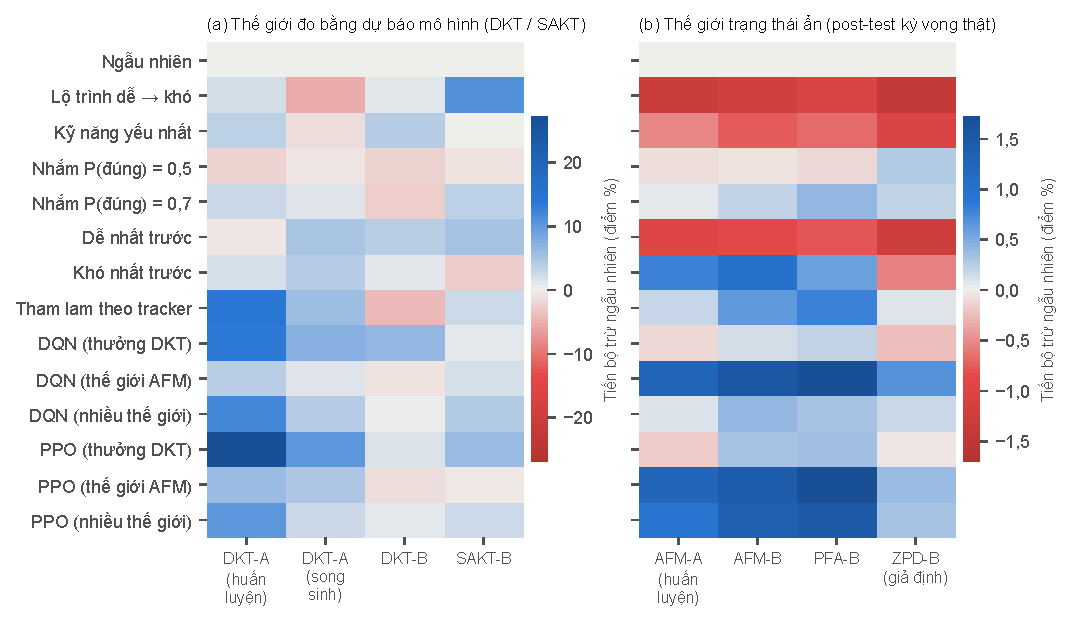
\includegraphics[width=\linewidth]{figures/fig_evaluation_matrix.pdf}
\caption{Tiến bộ so với chọn ngẫu nhiên trong từng thế giới. (a) Các thế giới đo bằng dự báo của chính một mô hình KT nơ-ron; (b) các thế giới có trạng thái ẩn đã biết. Ô xanh: tiến bộ post-test mô phỏng nhiều hơn ngẫu nhiên; ô đỏ: ít hơn. Thang màu của hai panel khác nhau; giá trị và khoảng tin cậy 95\% có trong tệp bổ sung \texttt{evaluation\_matrix\_long.csv}.}
\label{fig:matrix}
\end{figure}

\subsection{H2 và H3: tiến bộ lớn được báo cáo ở nơi không thể có học}\label{sec:res-h2}

Trong thế giới đối chứng âm IRT-B, tiến bộ post-test thật của mọi chính sách đúng bằng 0 theo cách xây dựng. Dù vậy, tracker DKT triển khai vẫn báo tiến bộ {{phantom_greedy_kt}} điểm \% {{phantom_greedy_kt_ci}} cho bộ tối đa hóa tham lam, {{phantom_dqn_kt}} điểm \% {{phantom_dqn_kt_ci}} cho DQN và {{phantom_ppo_kt}} điểm \% {{phantom_ppo_kt_ci}} cho PPO, ủng hộ H2 (\cref{fig:phantom}). Tiến bộ được báo cáo phụ thuộc mạnh vào chính sách: {{phantom_random}} điểm \% với chọn ngẫu nhiên và {{phantom_dqn_afm}} điểm \% với DQN huấn luyện trong thế giới AFM. Trên {{h3_n}} chính sách không phải oracle, tiến bộ trong bộ mô phỏng huấn luyện và tiến bộ ảo trong thế giới không học tương quan thứ hạng gần như hoàn hảo (Spearman $\rho$ = {{h3_rho}}), ủng hộ H3 (\cref{fig:insim}): thứ hạng mà đánh giá trong mô phỏng tiêu chuẩn tạo ra về cơ bản là thứ hạng của mức học mà tracker gán cho các lựa chọn bài của chính sách khi thực tế không có học. Các mô hình khác fit trên A ít bị ảnh hưởng hơn nhiều (thăm dò; \cref{tab:observers}): trong IRT-B, AFM và PFA báo tiến bộ tối đa {{obs_afm_max}} và {{obs_pfa_max}} điểm \% với bất kỳ chính sách nào trong số này, còn mô hình IRT tĩnh báo từ {{obs_irt_min}} đến {{obs_irt_max}} điểm \%, tức gần như không có.

\begin{figure}[t]
\centering
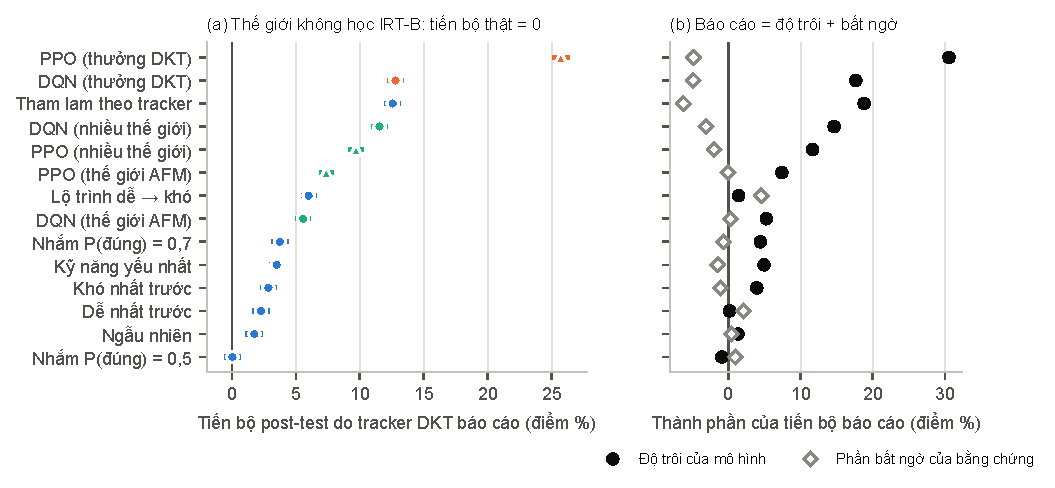
\includegraphics[width=\linewidth]{figures/fig_phantom_gain.pdf}
\caption{Đối chứng âm. (a) Tiến bộ post-test do tracker DKT báo cáo trong thế giới không học IRT-B, nơi tiến bộ thật của mọi chính sách bằng 0 (khoảng tin cậy 95\%). (b) Phân rã chính xác tiến bộ báo cáo thành độ trôi của tracker và phần bất ngờ của bằng chứng (phương trình \eqref{eq:decomposition}).}
\label{fig:phantom}
\end{figure}

\begin{figure}[t]
\centering
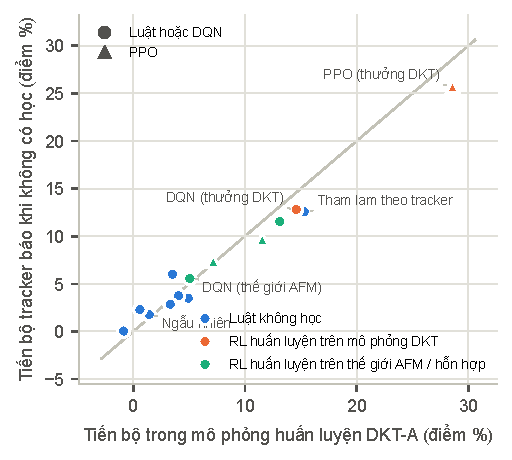
\includegraphics[width=0.62\linewidth]{figures/fig_in_sim_vs_phantom.pdf}
\caption{Tiến bộ trong mô phỏng DKT-A so với tiến bộ ảo mà tracker báo cáo trong thế giới không học IRT-B cho {{h3_n}} chính sách (Spearman $\rho$ = {{h3_rho}}). Đường chéo xám là $y=x$; hình tam giác là các tác tử PPO.}
\label{fig:insim}
\end{figure}

\subsection{H4: tiến bộ ảo đến từ đâu}\label{sec:res-h4}

Phép phân rã \eqref{eq:decomposition} quy tiến bộ ảo cho độ trôi: trong IRT-B, thay đổi dự báo mà tracker tự kỳ vọng cộng lại bằng {{drift_irt_ppo_kt}} điểm \% với PPO, {{drift_irt_dqn_kt}} điểm \% với DQN và {{drift_irt_greedy_kt}} điểm \% với bộ tối đa hóa tham lam, bị bù trừ một phần bởi phần bất ngờ âm vì thế giới kém thuận lợi hơn tracker kỳ vọng. Mức học ngầm định của một lần luyện phân tán mạnh hơn nhiều ở các mô hình nơ-ron so với các mô hình có số hạng học tường minh (\cref{fig:implied}): độ lệch chuẩn của độ trôi theo bài là {{sd_drift_dktA}} điểm \% với DKT, {{sd_drift_dkt2A}} với bản song sinh và {{sd_drift_saktA}} với SAKT, so với {{sd_drift_afmA}} với AFM, {{sd_drift_pfaA}} với PFA và đúng {{sd_drift_irtA}} với IRT, như \cref{prop:nodrift} đòi hỏi. Hiệu DKT--AFM là {{h4}} điểm \% {{h4_ci}}, ủng hộ H4. Trong các phân tích thăm dò, hai DKT — vốn dự báo tốt ngang nhau — chỉ đồng ý yếu về việc bài nào ``dạy'' được (Spearman $\rho$ = {{twin_rho}} {{twin_rho_ci}}), và độ trôi của DKT cao hơn ở các bài được làm nhiều ($\rho$ = {{expl_support_fraction}}) và các bài dễ hơn ($\rho$ = {{expl_irt_difficulty}} với độ khó IRT) nhưng không liên quan tới vị trí điển hình trong môn học ($\rho$ = {{expl_course_position}}).

Dọc theo mười tương tác thật tiếp theo của chính người học ({{lc_n}} người học; thăm dò), dự báo post-test của tracker trung bình chỉ dịch chuyển {{lc_tracker_gain}} điểm \%, dù trị tuyệt đối của dịch chuyển trung bình là {{lc_tracker_gain_abs}} điểm \%, so với {{lc_claimed_irt_A_abs}} điểm \% của IRT. Như vậy trên các chuỗi mà người học thật sự đi qua, độ trôi của DKT phần lớn tự triệt tiêu; chỉ khi một chính sách chọn bài vì độ trôi của chúng thì độ trôi mới cộng dồn thành tiến bộ hai chữ số.

\begin{figure}[t]
\centering
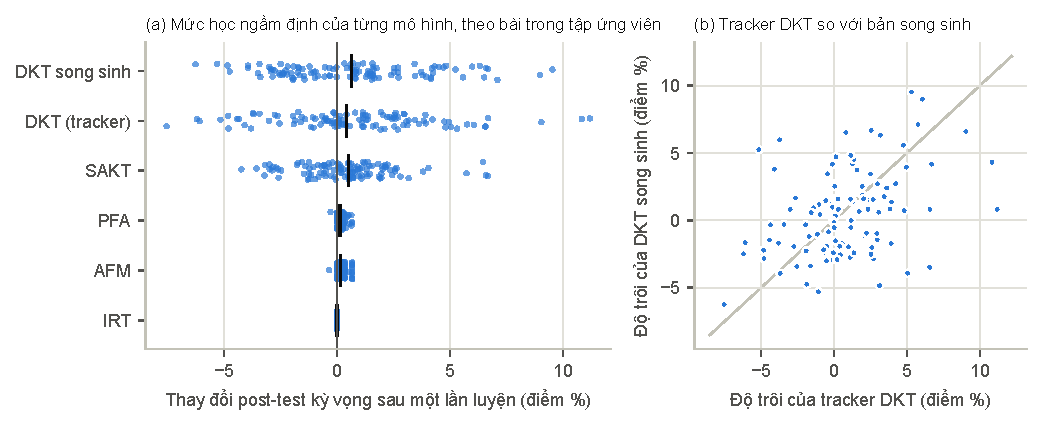
\includegraphics[width=\linewidth]{figures/fig_implied_learning.pdf}
\caption{Mức học ngầm định của từng mô hình. (a) Thay đổi post-test kỳ vọng sau một lần luyện mỗi bài trong tập ứng viên (độ trôi), trung bình trên 300 trạng thái xuất phát; vạch dọc là trung vị. (b) Độ trôi của tracker DKT so với bản song sinh huấn luyện lại (Spearman $\rho$ = {{twin_rho}}); đường chéo xám là $y=x$.}
\label{fig:implied}
\end{figure}

\subsection{Thăm dò: chính sách nào chuyển giao được}\label{sec:res-latent}

Trong các thế giới trạng thái ẩn, khoảng cách giữa các chính sách nhỏ nhưng nhất quán (\cref{fig:effort}). Tác tử huấn luyện trong thế giới AFM là các chính sách không đặc quyền tốt nhất: trong AFM-B, DQN huấn luyện với AFM đạt {{gain_afmB_dqn_afm}} điểm \% và PPO {{gain_afmB_ppo_afm}} điểm \%, so với {{gain_afmB_random}} điểm \% của chọn ngẫu nhiên và {{gain_afmB_oracle}} điểm \% của oracle một bước có đặc quyền; trong PFA-B, các giá trị tương ứng là {{gain_pfaB_dqn_afm}}, {{gain_pfaB_ppo_afm}}, {{gain_pfaB_random}} và {{gain_pfaB_oracle}} điểm \%. Trong thế giới độ khó mong muốn giả định ZPD-B, khoảng cách nhỏ hơn ({{gain_zpdB_dqn_afm}} và {{gain_zpdB_ppo_afm}} so với {{gain_zpdB_random}} điểm \%). Lợi thế so với ngẫu nhiên trong trường hợp xấu nhất trên ba thế giới ẩn là {{wc_dqn_afm}} điểm \% với DQN và {{wc_ppo_afm}} điểm \% với PPO, lớn nhất trong mọi chính sách, trong khi các tác tử thưởng KT có trường hợp xấu nhất {{wc_dqn_kt}} và {{wc_ppo_kt}} điểm \%; PPO huấn luyện trên nhiều thế giới đạt gần như vậy ({{wc_ppo_mix}} điểm \%). Tác tử huấn luyện với AFM cũng cần ít lượt nộp thêm hơn ({{extra_afmB_dqn_afm}} và {{extra_afmB_ppo_afm}} lượt trên mười bài trong AFM-B, so với {{extra_afmB_random}} của chọn ngẫu nhiên).

Độ bền này có giới hạn rõ ràng. AFM-B, PFA-B và ZPD-B có chung cấu trúc logistic cộng với thế giới huấn luyện AFM, nên việc chuyển giao giữa chúng một phần là do cách xây dựng. Trong các thế giới nơ-ron, vốn không chia sẻ cấu trúc đó, lợi thế so với ngẫu nhiên của các tác tử huấn luyện với AFM dao động từ {{rob_min_neural_afm}} đến {{rob_max_neural_afm}} điểm \% và âm trong DKT-B ({{rob_dqn_afm_dktB}} và {{rob_ppo_afm_dktB}} điểm \%). Các luật nhắm xác suất đúng dự báo 0,7 nhỉnh hơn ngẫu nhiên ở mọi thế giới ẩn (trường hợp xấu nhất {{wc_zpd70}} điểm \%), trong khi lộ trình dễ$\to$khó và luật chọn bài dễ nhất trước luôn kém nhất trong các thế giới ẩn, vì dành lượt luyện cho những bài người học vốn đã giải được.

\begin{figure}[t]
\centering
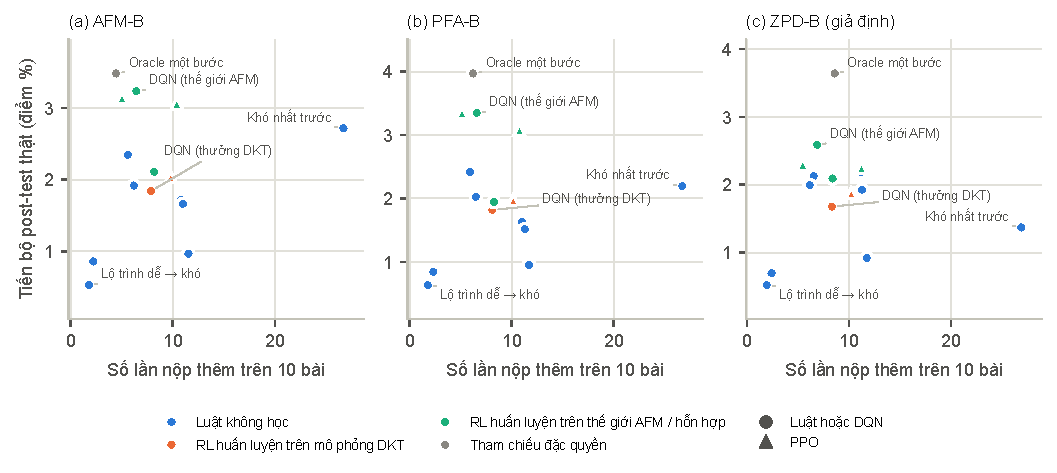
\includegraphics[width=\linewidth]{figures/fig_gain_effort.pdf}
\caption{Tiến bộ post-test thật so với số lượt nộp thêm trên mười bài trong ba thế giới ẩn fit hoặc xây dựng từ phân vùng B: (a) AFM-B, (b) PFA-B và (c) thế giới độ khó mong muốn giả định ZPD-B. Màu phân biệt các họ chính sách, hình tam giác đánh dấu tác tử PPO.}
\label{fig:effort}
\end{figure}
